\section{Sensoren}
Die Wetterstation Arbon verfügt über vier Sensoren bzw. Sensor-Einheiten: Webcam, Kombi-Wetter-Transmitter, Wassertemperatur-Sensor und Pegelsensor. Auf der Plattform im See draussen befindet sich lediglich ein Schaltschrank mit Datenwandlern und keine Auswerteeinheit. Sämtliche Daten werden per TCP/IP an den Server geschickt. Abbildung \ref{img:schaltschrank} zeigt den schematischen Aufbau der Komponenten im Schaltschrank und die angeschlossenen Sensoren. Die Stromversorgung ist der Übersicht halber nicht dargestellt.

\begin{figure}[h]
	\centering
	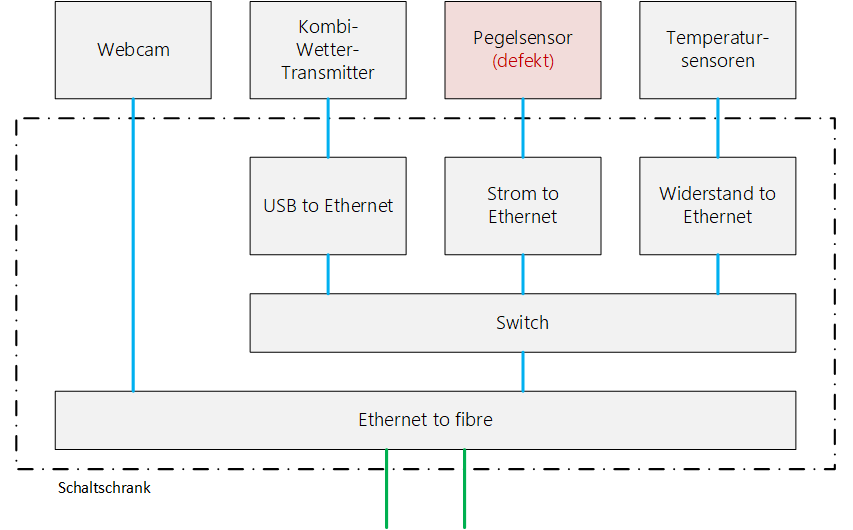
\includegraphics[width=0.9\linewidth]{img/schaltschrank.pdf}
	\caption{Hardware-Aufbau der Wetterstation Arbon}
	\label{img:schaltschrank}
\end{figure}



\subsection{Pegelmesser}
Der bisherige Pegel-Sensor nutzte das Prinzip der hydrostatischen Druckmessung. Der Sensor ist nun aber defekt und muss ersetzt werden. Neben der hydrostatischen Druckmessung kommen weitere potentielle Messprinzipien in Fragen. Sie alle erfüllen die Grundanforderung bezüglich Messdistanz und Robustheit. Während der Bachelor-Arbeit wird der passende Pegelsensor getestet und ausgewählt. Möglich ist:

\begin{itemize}  
\item Hydrostatische Druckmessung
\item Ultraschall-Distanzmessung
\item Radar-Distanzmessung
\item Time-of-flight-Distanzmessung
\end{itemize}

\subsection{Wassertemperatursensoren}
Die Wassertemperatur wird definitionsgemäss einen Meter unterhalb der Wasseroberfläche gemessen. Die Wetterstation Arbon verwendet eine Reihe von acht PT100-Widerständen. Diese sind in einem Kunststoffrohr im Abstand von 50~cm angeordnet. Abhängig vom gemessenen Pegel kann so der richtige Temperatursensor für die Wassertemperatur ausgewählt werden. 
\newline

\noindent
%\subsection*{Problem: Defekter Widerstand}
Von den acht verbauten Sensoren ist einer defekt. 
\newline

\noindent
%\subsection*{Lösungsansatz}
Da die Reparatur allerdings sehr aufwändig ist, und der Wert durch die beiden Nachbarwiderstände interpoliert werden kann, wird der Widerstand nicht ersetzt. Für uns besteht diesbezüglich kein Handlungsbedarf.












